%!TEX root = /Users/zolkko/Projects/zolkko-alarm/doc/main.tex
\section{Анализ современных систем автоматизированного проектирования программно-аппаратных микроконтроллерных комплексов}

\subsection{Общие сведения о САПР}
\begin{par}
САПР --- Система автоматизированного проектирования --- автоматизированная система, реализующая
информационную технологию выполнения функций проектирования, представляет собой
организационно-техническую систему, предназначенную для автоматизации процесса проектирования,
состоящую из персонала и комплекса технических, программных и других средств
автоматизации его деятельности.
\end{par}

\begin{par}
На некотором этапе своего развития системы проектирования претерпели качественное изменение.
Оно было связано с тем, что САПР из набора каким-то образом связанных между собой прикладных
программ начали превращаться в мобильные и стройно организованные системы, способные к
настройке на особенности предметной области и на требования конечного пользователя,
допускающие расширение функциональных возможностей за счёт сравнительно несложного подключения
новых прикладных программных модулей и обеспечивающих поддержку групповой разработки сложных схем
коллективом проектировщиков.
\end{par}

\begin{par}
Особенное значение САПР приобрели в микроэлектронике, поскольку современная радиоэлектронная аппаратура базируется на применении сверхбольших интегральных схем, разработка которых без применения САПР невозможна или крайне затруднительна.
\end{par}

\begin{par}
Специализированные САПР для разработки электронных устройств и печатных плат получили название
Electronic Design Automation - EDA, автоматизация проектирования электронных приборов.
Комплексы такого типа зачастую позволяют создавать принципиальные электрические схемы схемы с
помощью графического интерфейса, создавать и модифицировать  базу радиоэлектронных компонентов,
проверять целостность сигналов на ней и проводить аналоговое и цифровое моделирование
разрабатываемого устройства ещё на этапе проектирования.
\end{par}


\subsubsection{Обзор Electric VLSI}
\begin{par}
Electric VLSI --- cистема автоматизированного проектирования сверхбольших интегральных схем, используемая для разработки электрических схем и проектирования
топологии печатных плат и интегральных схем.
\end{par}
\begin{par}
Electric являлся open-source проектом, разработка
которого в течении многих лет поддерживалась\cite{electric} компанией Sun Microsystems,
а в настоящее время курируется компанией Oracle. \\*
Наиболее ценная встроенная в Electric возможность —-- это система привязок,
которая даёт возможность осуществлять проектирование сверху вниз с соблюдением целостности
всех соединений.
\end{par}

\subsubsection{Обзор Proteus VSM}
\begin{par}
Proteus VSM --- пакет программ для автоматизированного проектирования электронных схем.
    Разработка компании Labcenter Electronics.
\end{par}
\begin{par}
Proteus VSM сочитает в себе функциональность SPICE симуляции электронных цепей,
анимированные компоненты, модели микропроцессоров и средства симуляции сложных
микроконтроллерых решений. Это первая система сочетающая в себе все эти особенности
и позволяющая разработать и протестировать решение до создания прототипа устройства.
Такое тестирование осуществляется за счёт взаимодействия с отображаемыми и анимированными
виртуальными устройствами такими как свето-диоды, LCD, кнопки и переключатели.
При этом симуляция производится в режиме блиском к режиму реального времени.
Так производительности 1 ГГц Pentium III ЭВМ будет достаточно для симуляции работы
микропроцессора 8051 на частоте 12 МГц в режиме реального времени. Так же Proteus VSM
предоставляет экстенсивные средства отладки, включая точки останова, трассировку и вывод
значений  переменных микропрограмм как для машинных кодов, так и для языков высокого
уровня. Proteus VSM  включает несколько виртуальныхинструментов: осцилограф, логический
анализатор, генератор функций, генератор по шаблонам, виртуальный терминал, отладчики SPI
и I2C интерфейсов , а так же простые инструменты как вольтметр и амперметр, существенно
облегчающих анализ и отладку схемы.
\end{par}
\begin{par}
В дополнении к моделям микропроцессоров в Proteus VSM так же включена большая библиотека
стандартных пассивных и акивных моделей устройств.
\end{par}
\begin{par}
Пакет Proteus состоит из двух частей, двух подпрограмм: ISIS – программа синтеза и
моделирования непосредственно электронных схем и ARES – программа разработки печатных
плат.

\begin{figure}[h]
	\center{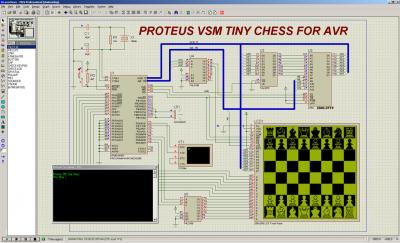
\includegraphics[bb=0 0 400 243, clip, scale=0.8]{proteus.png}}
	\caption{Главное окно программы Proteus ISIS}
	\label{img:proteus}
\end{figure}

\end{par}

\subsubsection{Обзор KiCAD}
\begin{par}
KiCad --- распространяемый по лицензии GNU General Public License программный
комплекс класса EDA с открытыми исходными текстами, предназначенный для разработки
электрических схем и печатных плат. \\*
Кроссплатформенность компонентов KiCad обеспечивается использованием библиотеки wxWidgets.
Поддерживаются операционные системы Linux, Windows NT 5.x, FreeBSD и Solaris.
\begin{figure}[h]
	\center{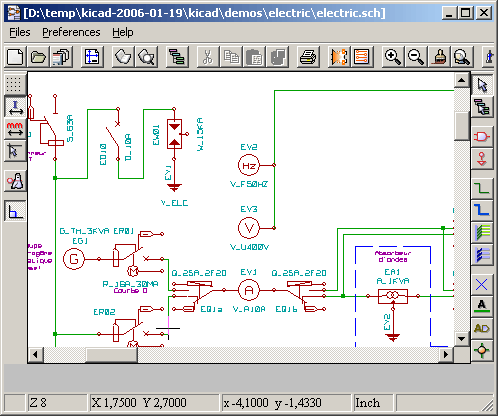
\includegraphics[bb=0 0 498 416, clip, scale=0.5]{kicad.png}}
	\caption{Главное окно программы KiCAD Eeschema}
	\label{img:kicad}
\end{figure}
\end{par}

\begin{par}
В состав KiCAD входят программы:
    \begin{itemize}
        \item{}kicad --— менеджер проектов;
        \item{}eeschema —-- редактор электрических схем (рис. \ref{img:kicad});
        \item{}встроенный редактор символов схем (библиотечных компонентов);
        \item{}pcbnew --— редактор печатных плат;
        \item{}встроенный редактор образов посадочных мест (библиотечных компонентов);
        \item{}3D Viewer --— 3D-просмотрщик печатных плат на базе OpenGL (часть pcbnew);
        \item{}gerbview --— просмотрщик файлов Gerber (фотошаблонов);
        \item{}cvpcb --— программа для выбора посадочных мест, соответствующих компонентам на схеме;
        \item{}wyoeditor --— текстовый редактор для просмотра отчетов.
    \end{itemize}
\end{par}


\subsubsection{Обзор gEDA}
\begin{par}
gEDA --- набор программного обеспечения для проектирования электронных устройств,
распространяемый по лицензии GPL. Включает в себя инструменты для редактирования
электрических схем, симуляции цифровых и аналоговых схем, трассировки печатных плат
и подготовки к производству. Проект изначально ориентирован на UNIX-совместимые
платформы, хотя некоторые программы, входящие в его состав, в настоящее время
портированы под ОС Windows\cite{geda}.
\end{par}
\begin{par}
В настоящее время пакет вполне пригоден для проектирования устройств среднего уровня
сложности и может быть полезен как студентам, любителям, так и профессиональным
разработчикам электронных устройств.
\end{par}
\begin{par}
За время существования проекта, к нему примкнуло несколько самостоятельных
узкоспециализированных проектов, которые теперь считаются частью gEDA, в
связи с чем оригинальный проект и его составные части стали называть
gEDA/gaf (gschem and friends) (рис. \ref{img:geda}).
\begin{figure}[h]
	\center{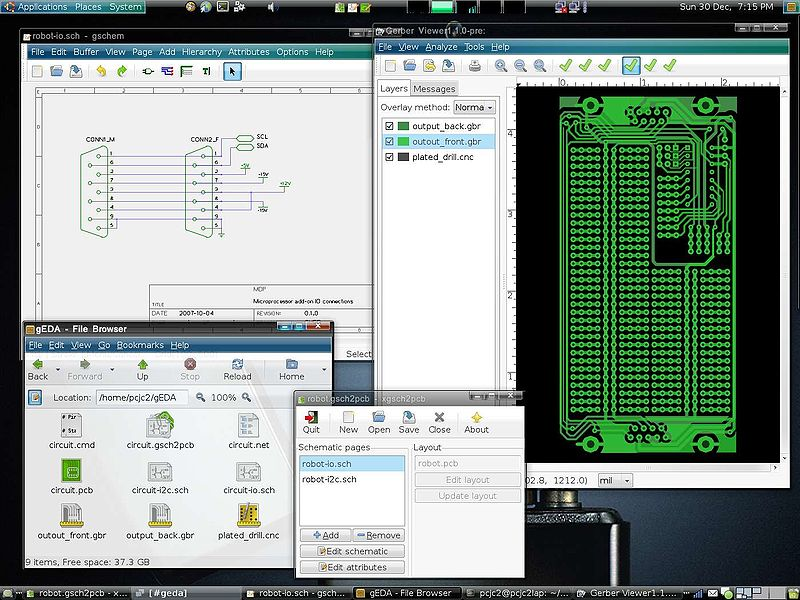
\includegraphics[bb=0 0 800 600, clip, scale=0.3]{geda.png}}
	\caption{gEDA}
	\label{img:geda}
\end{figure}
\end{par}

\subsubsection{Обзор Eagle EDA}
\begin{par}
EAGLE это лёгкий в использовании, но достаточной мощный EDA пакет, разрабатываемый немецкой компанией CadSoft.
В состам системы входят:
\begin{enumerate}
	\item{}Layout Editor --- пограмма для проектирования печатных плат (рис. \ref{img:eagle_brd}). 
		\begin{itemize}
			\item{}Максимальная рабочая поверхность 1.6 x 1.6м;
			\item{}разрешение - 1/10,000мм (0.1 микрон);
			\item{}до шестнадцати сигнальных слоёв;
			\item{}большая библиотека компонентов;
			\item{}copper pouring - области на печатной плате заполненные  медью, что часто используется для создания областей <<земли>> и уменьшения необходимого травильного вещества при производстве;
			\item{}встроенная ДРЦ проверка.
		\end{itemize}
        \begin{figure}[h]
            \center{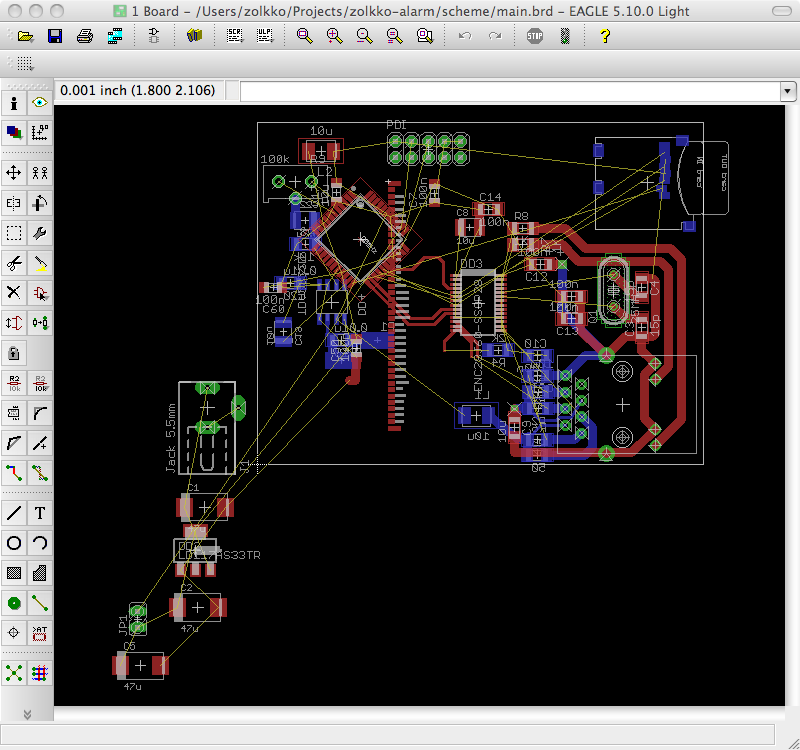
\includegraphics[bb=0 0 800 800, clip, scale=0.3]{eagle_brd.png}}
            \caption{Окно редактора печатных плат Eagle}
            \label{img:eagle_brd}
        \end{figure}

	
	\item{}Schematic Editor - программа для создания принципиальных электрических схем (рис. \ref{img:eagle_sch}).
		\begin{itemize}
			\item{}до 999 листов на одну схему;
			\item{}проверка эллектичских правил;
			\item{}обмен вентелей и пинов;
			\item{}возможность создания печатной платы из схемы одной командой.
		\end{itemize}
        \begin{figure}[h]
            \center{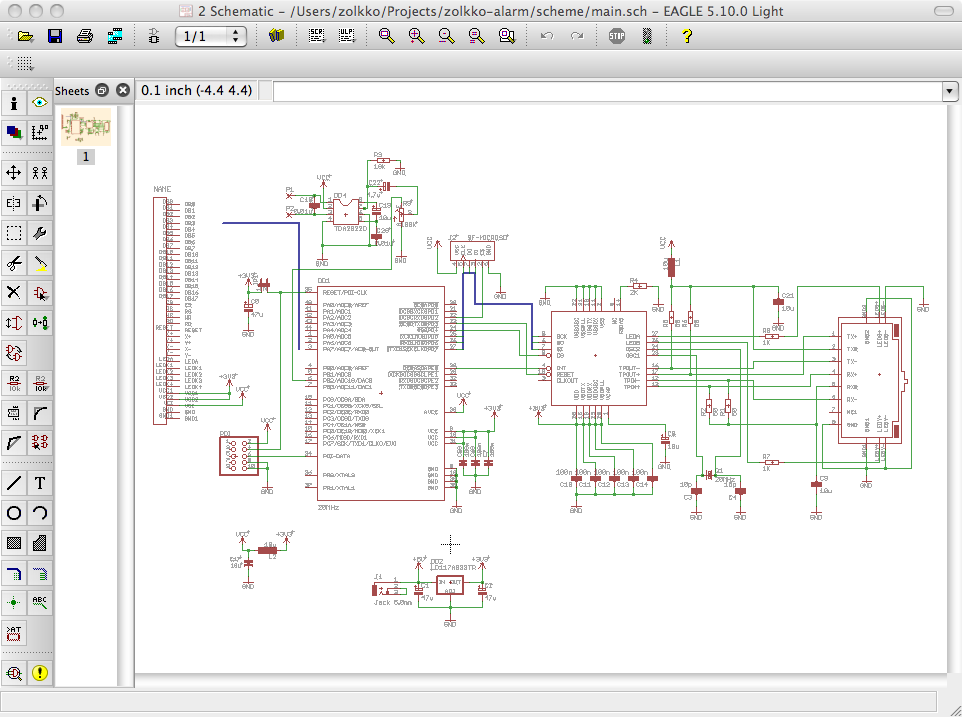
\includegraphics[bb=0 0 1010 730, clip, scale=0.3]{eagle_sch.png}}
            \caption{Окно редактора пренципиальных схем Eagle}
            \label{img:eagle_sch}
        \end{figure}
	\item{}Autorouter - программа автоматической трассировки.
		\begin{itemize}
			\item{}ripup-and-retry трассировщик - на первом проходе выполняется соединение абсолютно всех проводников без обращения внимания на возможные конфликты, заключающиеся в пересечении проводников на одном слое и нарушении зазоров. На каждом последующем проходе автотрассировщик пытается уменьшить количество конфликтов, разрывая и вновь прокладывая связи;
			\item{}до шестнадцати сигнальных слоёв;
			\item{}стратегия трассировки может быть подстроена заданием весовых коэфициентов.
		\end{itemize}
\end{enumerate}

Все эти программы встроены в один пользовательский интерфейс, таким образом нет необходимости в
предварительном конвертировании нет-листов.
\end{par}


\subsection{Обзор современных систем программирования микроконтроллеров}

Ведущими разработчиками 8/16 битных микроконтролеров на сегодняшний день
являются компании:
\begin{itemize}	
	\item{} Microchip Technology Inc. -- выпускающие микроконтроллеры семейства PIC и
		сигнальные микроконтроллеры dsPIC,
		получивших широкое распространение в странах серевной и южной америки.
		Отличительной особенностью PIC--контроллеров является хорошая преемственность
		различных семейств.
		8-битные микроконтроллеры представлены двумя базовыми архитектурами ядра:
		BASELINE и MID-RANGE. Основным инструментом разработки является среда программирования
		MPLab и набор компиляторов GCC.
	\item{} STMicroelectronics -- европейская компания, активно продвигающая свои 8 и 32
		разрядные микроконтроллеры на рынке. В качестве среды разработки предлагается
		использовать адаптированную версию набора компиляторов GCC.
	\item{} Texas Instruments --специализирующаяся на выпуске цифровых сигнальных процессоров
		и наиболее удачной линейки микроконтрллеров общего назначения MSP430.
	\item{} NXP Semiconductors -- производит 8 разрядные микроконтроллеры
			80C51: LPC900 и LPC700.
			Основным инструментом разработчика является адаптированная версия
			Keil PK51 Professional Developers Kit, предоставляющей инструменты для
			генерации программ для LPC, и включающая в себя среду разработки
			$\mu{}$Vision IDE, C51 ANSI C компилятор и A51 макро ассемблер, $\mu{}$Vision отладчик
			со встроенным симулятором ЦПУ и переферийных устройств. В комплект поставки
			среды так же входит внутрисхемный отладчик ISD51.			
	\item{} Freescale Semiconductor -- HC80, HC05, HC11.
	Эти микроконтроллеры используют расширенную архитектуру ЦПУ M68HC08.
	Основным иструментом разработки является CodeWarrior Development Studio, в поставку
	которой так же включается симулятор чипа и мастер автоматического генерирования
	кода ''Processor Expert''.
	\item{} Atmel Corporation -- выпускает микроконтроллеры AVR, основанные на ядре
	собственной разработки. Основное средство разработки -- AVR Studio. В начале 2011
	года компания прекратила поддержку старых версий AVR Studio 4 и AVR Studio 32,
	заместив их AVR Studio 5 -- средой разработки основанной на Microsoft Visual
	Studio Shell. В качестве компилатора выступает адаптированная версия GCC. Так
	же в комплекте среды разработки поставляется симулятор ЦПУ и переферии, и
	набор программного обеспечения ''AF''.
\end{itemize}

Таким образом, все лидирующие производители микроконтроллеров предоставляют
бесплатные системы программирования своих мкроконтроллеров.
Причём, можно отметить, что системы программирования либо основанны на коде 
набора компиляторов GNU GCC, либо в качестве стандартной среды разработки лицензируется
программное обеспечение других компаний. Во втором случае, зачастую, бесплатные
стандартные системы программирования обладают рядом ограничений, позволяющим только
опробовать демонстрационные проекты.

Однако, на рынке пристствует довольно большео число компаний специализирующихся
исключительно на создании систем программирования для встраиваемых систем. Лидером
в этой области является IAR Systems -- компания предоставляющая широчайший перечень компиляторов и стандартных библиотек для большого числа микроконтроллеров разных архитектур.
Их продукт IAR Embedded Workbench поддерживает следующие семейства микроконтроллеров:
\begin{itemize}
	\item{} 8051;
	\item{} ARM;
	\item{} Atmel AVR, AVR32;
	\item{} Freescale ColdFire, Freescale S08, Freescale HCS12;
	\item{} Maxim MAXQ;
	\item{} Microchip dsPIC/PIC24, PIC18;
	\item{} National CR16C;
	\item{} Renesas RL78, 78K, V850, H8, M16C, R8C, M32C, RX, R32C, SuperH;
	\item{} Samsung SAM8;
	\item{} STMicroelectronics STM8;
	\item{} TI MSP430.
\end{itemize}
Ещё одним интерестным продуктом этой компании является IAR visualState -- системе
программирования, автоматически генерирующей программный код на основе графически
заданного конечного автомата. При этом возможно проводить комдинированную разработку
программного обеспечения, когда часть кода программы генерируется автоматически, а часть
разрабатывается программистом.

\begin{figure}[h]
	\center{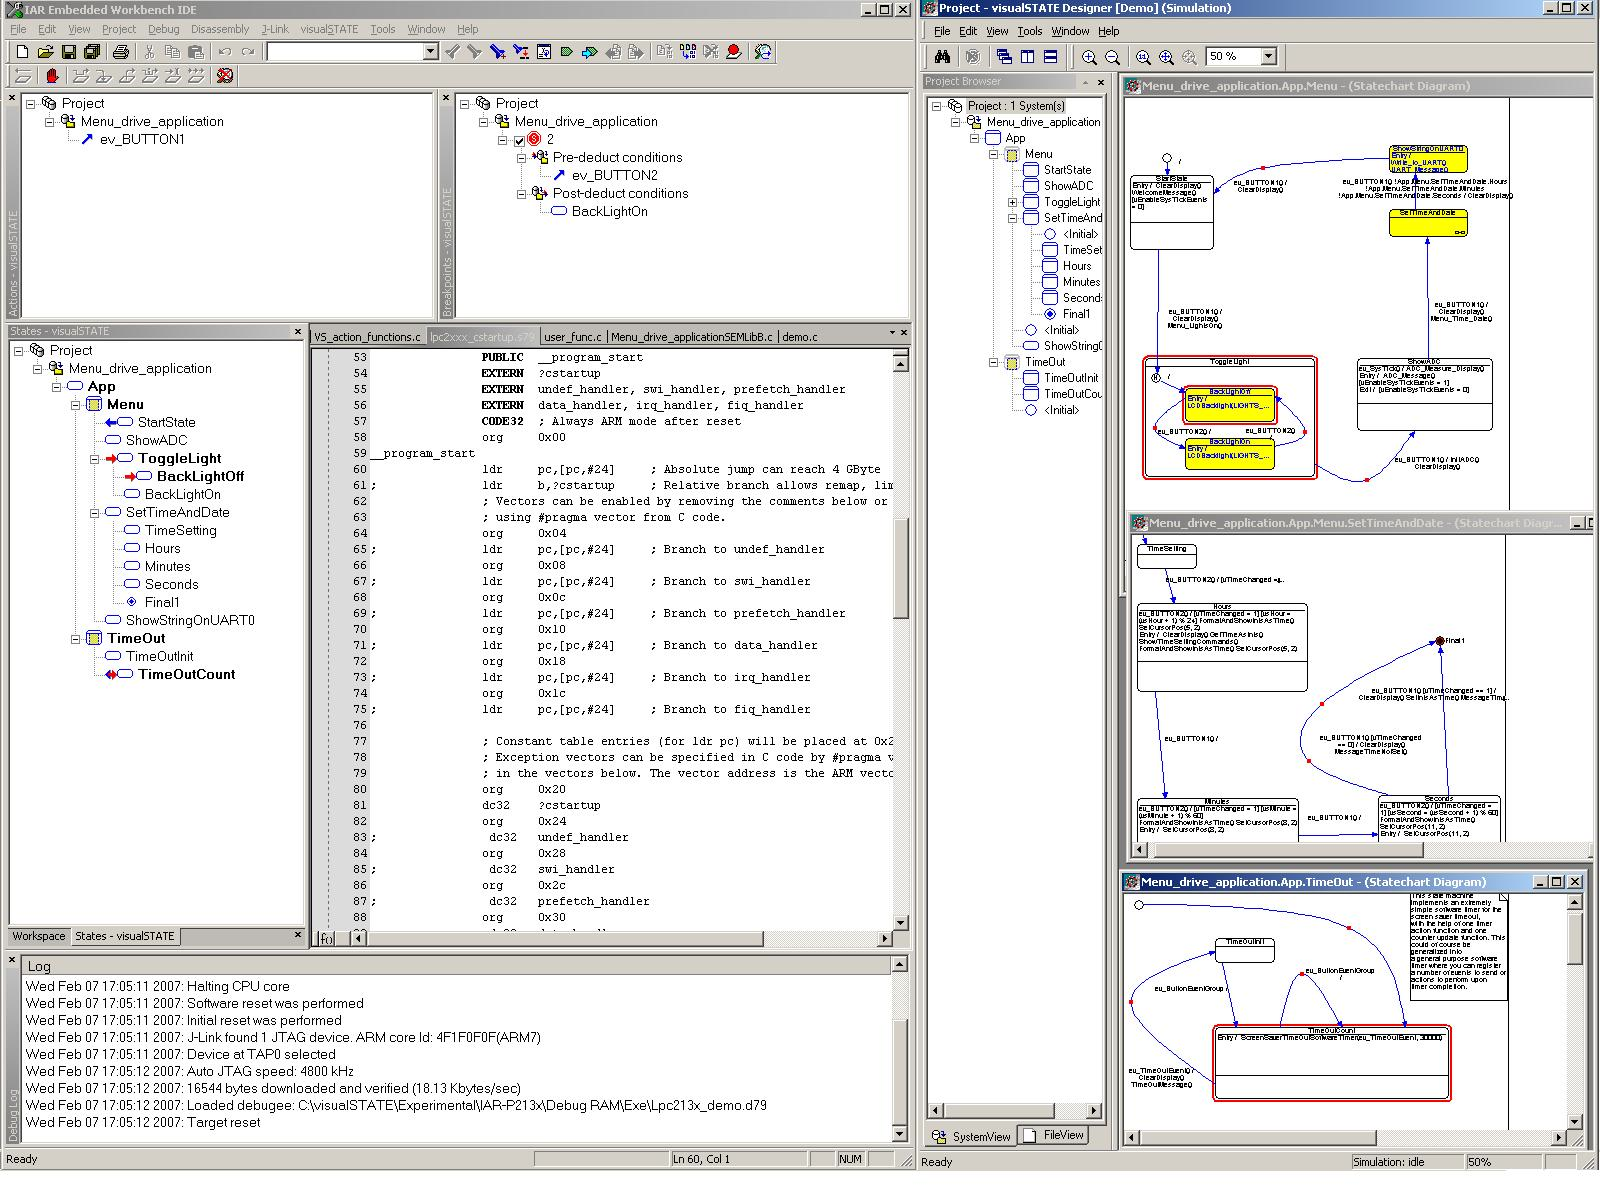
\includegraphics[bb=0 0 900 700, clip, scale=0.3]{iar_vis_state.png}}
	\caption{Среда разработки IAR visualSTATE}
	\label{img:iarVis}
\end{figure}

\newpage{}

